\documentclass{article}
\usepackage[margin=0.75in]{geometry}
\usepackage{amsmath}
\usepackage{physics}
\usepackage{listings}
\usepackage{caption}
\usepackage{graphicx}
\usepackage{algorithm}
\usepackage{algpseudocode}
\usepackage{amsfonts}
\usepackage{array}
\usepackage{subfig}
\graphicspath{{../Images/}}


\newcommand{\pset}[2]{
\pagestyle{myheadings}
    \thispagestyle{plain}
    \newpage
    \setcounter{page}{1}
    \noindent
    \begin{center}
    \framebox{
        \vbox{\vspace{2mm}
        \hbox to 6.28in { {{\bf #1} \hfill  \textbf{\today}}}
        \vspace{4mm}
        \hbox to 6.28in { {\Large \hfill Autocatalytic Reaction Networks from a Binary Vector Space Perspective \hfill} }
        \vspace{2mm}
        \hbox to 6.28in { {\hfill \it{Varun Varanasi}} \hfill }
        \vspace{2mm}}}
    \end{center}
    \markboth{First-Order Reaction Perspective}{First-Order Reaction Perspective}
    \vspace*{4mm}
\	}
\begin{document}


\title{RAF Networks from Binary Vector Space Perspective}
\author{Varun Varanasi}
\maketitle

\section{Introduction}

\subsection{Set Up}
Consider a Kauffman pre-biotic chemical model over the alphhabet $\{A,B\}$ with the following parameters:


\begin{center}
\begin{tabular}{ | c || c| } 
  \hline
  \textbf{Parameter} & \textbf{Definition} \\ 
  \hline
  n &  Maximum size of a molecule \\ 
  f &  Scaled probability parameter   \\ 
  t & Maximum size of food set \\ 
  \hline
\end{tabular}
\end{center}

From these parameters we can define the following variables:


\begin{center}
    \begin{tabular}{ | c || c| c|} 
      \hline
      \textbf{Variable} & \textbf{Name }& \textbf{Definition} \\ 
      \hline
      X & Molecule Set &  All possible combinations of $A,B$ under size length $n$ \\ 
      F & Food Set &  All possible combinations of $A,B$ under size length $t$  \\ 
      R & Reaction Set & All possible addition and division reactions that stay within the set X\\ 
      C & Catalyst Set & Catalyst relations between elements in X and R: $(x,r) \in C , x \in X, r \in R$  \\
      \hline
\end{tabular}
\end{center}

For a set network size $n$ we can think our autocatalytic set consisting of $X(n)$ molecules connected by $R(n)$ reactions. 
In the below visualization we differentiate between food set molecules(gold), non-food molecules (green), and reactions (red).
Arrows between nodes indicate reaction relations. 

\begin{figure}[h]%
    \centering
    \subfloat[\centering Empty Network]{{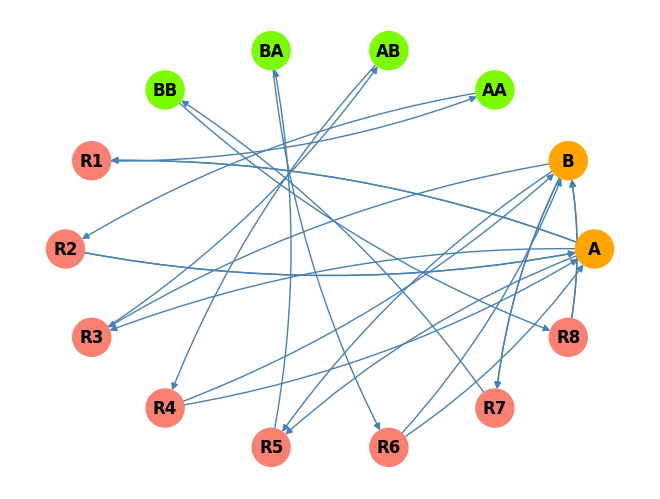
\includegraphics[width=8cm]{empty_network} }}%
    \qquad
    \subfloat[\centering Catalyzed Network]{{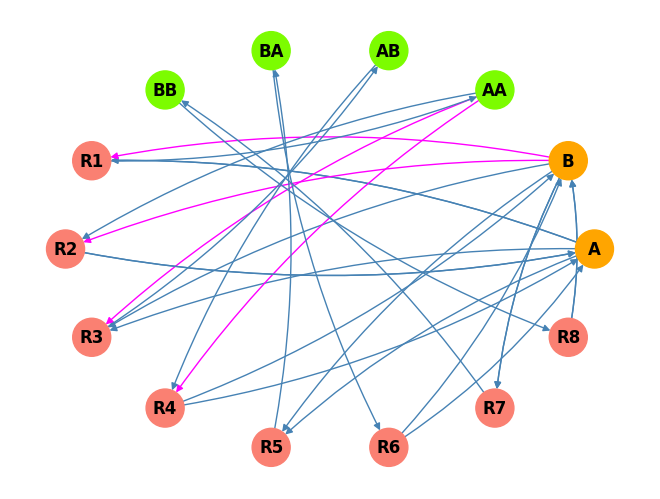
\includegraphics[width=8cm]{example_network} }}%
    \caption{Kauffman Network Visualizations}
\end{figure}

On this underlying structure, we can add catalysts to create a full kauffman network.
For the purposes of this model, we consider this occuring with a random probability p dictated by the parameter f.
Catalysts can be thought of as a relationship between a reaction and a molecule. 
Since for a given n, we consider the underlying structure to be constant, we can represent each unique Kauffman network in terms of its catalyzing relations.
We can therefore represent each Kauffman network as an adjacency matrix existing in $M^{X(n) \times R(n)}$.  \\

\subsection{RAF Sets}
\textbf{RAF Definition:} A Kauffman network is said to be Reflexivley Autocatalytic and Food generated if every reaction is catalyzed by a molecule involved in a reaction and every reactant can be constructed from the food set by repetead application of catalyzed reactions. \\

Limitations of the RAF Definition:
\begin{itemize}
    \item No restriction on a molecule catalyzing the reaction that produces it
\end{itemize}


\section{Probability Argument}

\subsection{RAF Cases}
A key observation is that any RAF set of catalysts can be seen as an RAF core, the portion of catalyzing reactions that are directly responsible for the self-sustaining properties, and additional catalyzing relations that are irrelvant or produce fringe molecules (molecules not used in the main reaction cycle).
If we hold our food set to be constant with size 2, we notice that an RAF set can occur via two ways: 

\begin{enumerate}
    \item \textbf{Internal RAF}: RAF set is contained within Food Set (Reactants, Products, and Catalysts are all in Food Set)
    \item \textbf{First-Order RAF}: RAF set contains a molecule produced via addition of Food Set molecules that does not exist within the food set.
\end{enumerate}

We refer to molecules produce as in described in 2) as first-order molecules. These are molecules that are created from a single reaction involving food set molecules. For example we classify the following reaction as first-order

$$
A + AB \rightarrow AAB
$$

since $AAB \notin F$. 
We further posit that the 2 cases outlined above are comprehensive of all RAF sets. 
Logically, any RAF set must be connected to the Food Set. This is either because the RAF set never leaves the food set or it passes through the set of first-order molecules. 
\textbf{Make this claim more rigorous}
This statement has also been verified across 10,000 trials and 5 different network sizes. \\


\subsection{Probability}

In our adjacency matrix framework of a Kauffman network, we understand this as every RAF networking containing a connection falling under the above criteria.
Alternatively, every non-RAF network will have no connections present in these categories.
In a standard network with $t = 2$, we find the following:

\begin{center}
    \begin{tabular}{ | c || c| c| } 
      \hline
      \textbf{RAF Type} & \textbf{Food Size}  & \textbf{Reaction Count}\\ 
      \hline
      Internal &  6 & 8 \\ 
      First-Order &  6 & 32 \\ 
      \hline
\end{tabular}
\end{center}

Therefore, in our representation of a random network $C \in M^{X \times R}$, we say that C is non-raf \textbf{if and only if} there are no connections between the Food set and the 40 reactions above.
We can therefore represent an arbitrary non-RAF network as

\begin{gather*}
M = \begin{bmatrix}
    0 & A \\
    B & C
\end{bmatrix} \\
A \in M^{ 6 \times R(n) - 40}, \quad B \in M^{X(n) - 6 \times  40}, \quad C \in M^{X(n) - 6 \times R(n) - 40}
\end{gather*}


If we were to make a proabilistic argument, under this framework $ P(\text{non-RAF})$ is equivalent to having a 0 in the block matrix designated above. 
With a probability of catalysis p, 

$$
P(\text{non-RAF}) = (1 - p)^{240}
$$


Consequently, 
$$
P(\text{RAF}) = 1 - P(\text{non-RAF}) = 1 - (1 - p)^{240}
$$

Recall, that $p$ is defined by the parameter $f$ by the relation $p = \frac{f}{R(n)}$.

\begin{gather*}
    P(\text{RAF}) = 1 - P(\text{non-RAF}) = 1 - \left(1 - \frac{f}{R(n)} \right)^{240} \\
\end{gather*}




\subsection{Computational Comparison}

We can compare our above theoretical comparison to experimental result:

\begin{figure}[h]%
    \centering
    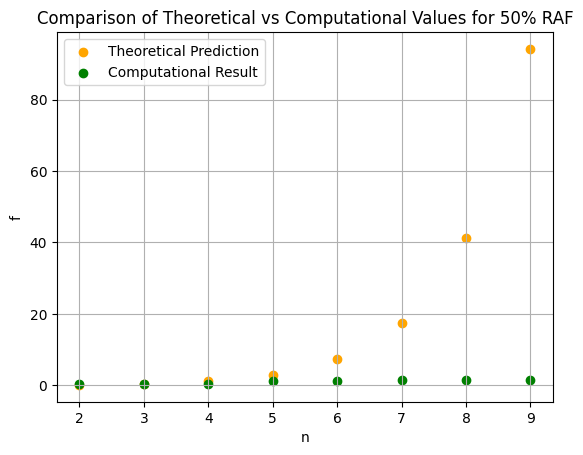
\includegraphics[width=8cm]{f_pred} 
\end{figure}

It is clear that our theoretical prediction is incorrect. \textbf{Why?}


\subsection{Geometric Interpretation}

If we think our block diagonal matrix as a vector existing in $F_2^X \times R$ we would expect the first 40 entires to be identically 0.
Geometrically, we imagine this as our data being concentrated along the axes in question.
Consequently, if we were to run PCA on a dataset of non-RAF sets, we would expect our principal components to correspond to these data axes. 
However, when we run this calculation, we do not find this to be true. 



\begin{center}
    \begin{tabular}{ | c || c| c|} 
      \hline
      \textbf{Network Size} & \textbf{Strongest Correlation Dimensions for first 3 Principal Components} & \textbf{Sample Size} \\ 
      \hline
      3 &  248, 426, 398 & 732 \\ 
      4 &  208, 1156, 1808 &  495\\ 
      5 &  13732,10908, 3456 &  222\\ 
      6 &  5908, 30084, 2766 &  391\\ 
      7 &  512, 1294, 560 &  78\\ 
      \hline
\end{tabular}
\end{center}

We also notice that many of our indicies are identically 0 in the datasets used. It is possible that the theoretical prediction is still accurate, but we have insufficient data to capture the behavior.
However, given the other evidence, it is likely that the theoretical prediction is inaccurate.



\section{Clustering Analysis}

\subsection{K-Nearest Neighbors}

\subsection{Agglomorative Heirarchical Clustering}

\end{document}